O \gls{lorawan}, é um protocolo de comunicação baseado na tecnologia \gls{lpwan}, que possui o objetivo de viabilizar a comunicação em grandes distâncias, conciliado ao baixo consumo energético.
O protocolo é open-source e mantido pela LoRa Alliance. 
Como citado anteriormente, a rede \gls{lorawan} é formada por dispositivos finais, getaways, servidores de rede e servidores de aplicação \cite{Camargo2022}. 

A figura~\ref{fig:stack_layer_lora} apresenta a pilha de elementos das camadas MAC e Física que compõem a arquitetura do protocolo \gls{lorawan}.

\begin{figure}[H]
    \centering
    \caption{Pilha de elementos das camadas LoRa/LoRaWan}
    \label{fig:stack_layer_lora}
    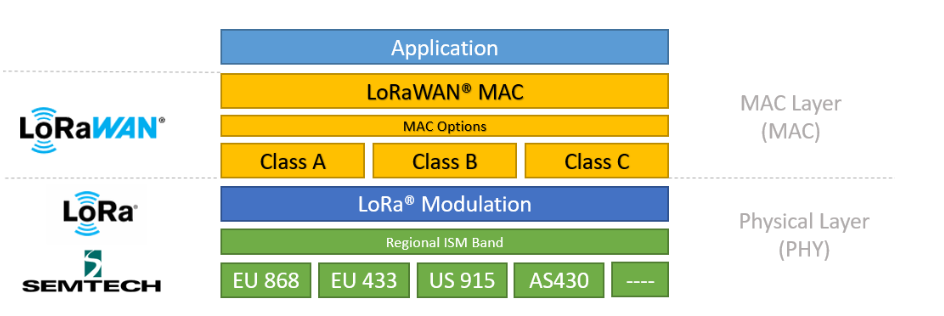
\includegraphics[width=0.85\textwidth]{sections/imagens/LoRaWan_Pilha_Camadas.png}
    \small
    \begin{quote}
        Fonte: Adaptado de Semtech Corporation \cite{semtech2024an1200_86}.
    \end{quote}
\end{figure}

\begin{figure}[H]
    \centering
    \caption{Implementação Típica de Rede LoRaWan}
    \label{fig:implementacao_tipica_lorawan}
    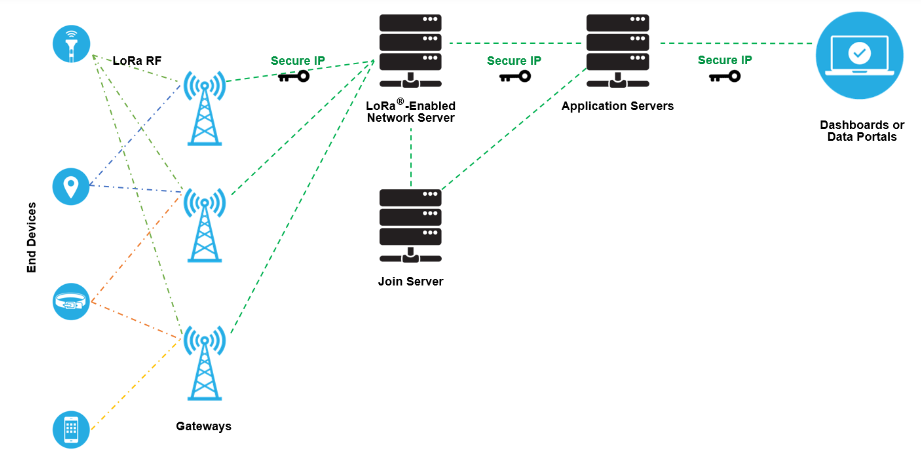
\includegraphics[width=0.85\textwidth]{sections/imagens/Implementacao_tipica_LoRaWan.png}
    \small
    \begin{quote}
        Fonte: Adaptado de Semtech Corporation \cite{semtech2024an1200_86}.
    \end{quote}
\end{figure}

A figura~\ref{fig:implementacao_tipica_lorawan} apresenta a arquitetura típica de uma sistema \gls{iot} que utiliza como base o protocolo \gls{lorawan} para viabilizar a comunicação entre os dispositivos. Cada elemento que compõe uma rede \gls{lorawan}, possui uma responsabilidade, tal qual, neste momento, é extremamente válido analisá-las individualmente:

\subsubsection{Dispositivos Finais (End Nodes)}

\citeonline{semtech2024an1200_86} define que dispositivos finais habilitados à LoRaWan são sensores ou atuadores que são conectados à gateways via modulação de rádio frequência LoRa. 

A maioria das aplicações desses dispositivos são autônomos, dependentes de baterias como fonte energética primária e possuem como responsabilidade digitalizar condições físicas como temperatura, captura de imagens, níveis de tremulação, entre outros.

Em relação às possíveis configurações que podem ser aplicadas nos dispositivos finais, como apresentado por \citeonline{Camargo2022}, cada nó pode assumir uma das configurações que a tabela~\ref{tab:tabela_classes} apresenta. Outro parâmetro configurável é o tipo de autenticação dos dispositivos em rede, onde há o padrão \gls{otaa}, onde o próprio dispositivo gerencia a conexão à rede e a \gls{abp}, onde os dispositivos são vinculados de forma manual à uma rede em específico, não passando por processo de entrada implementado no \gls{otaa}.

O LoRaWan utiliza o padrão AES de criptografia simétrica onde é aplicado tanto em camada de aplicação quanto em camada de rede.

Os dispositivos finais, corriqueiramente, são desenvolvidos sob microprocessadores, podendo tanto utilizar placas que já incluem módulos LoRaWan nativos, quanto serem desenvolvidos sob plataformas como ESP32, Arduíno, Raspberry Pi, entre outras.
A partir da construção do dispositivo, ou acoplamento de módulos, possibilita-se a captura de dados em ambiente \cite{Camargo2022}.

Como destacado por \citeonline{Sari2022} e \citeonline{Ahmad2021}, o ESP32 destaca-se nesse cenário como uma plataforma robusta de baixo custo, integrando conectividade sem fio e múltiplos modos de operação. 
Diferente de arquiteturas mais simples, o ESP32 permite a execução de tarefas complexas e segurança criptográfica sem comprometer severamente o ciclo de vida da bateria, desde que devidamente configurado.

Segundo \citeonline{Ferreira2020}, a vida útil da bateria é influenciada criticamente não apenas pelo hardware, mas pela eficiência das rotinas de escrita em periféricos e pela otimização do firmware.
Diante de tal afirmação destaca-se a função \textit{deep sleep} presente no ESP32 que possui como foco a minimização do consumo energético quando em estado ocioso.

\begin{figure}[H]
    \centering
    \caption{Módulo ESP32-CAM integrado com LoRa}
    \label{fig:esp32cam_lora}
    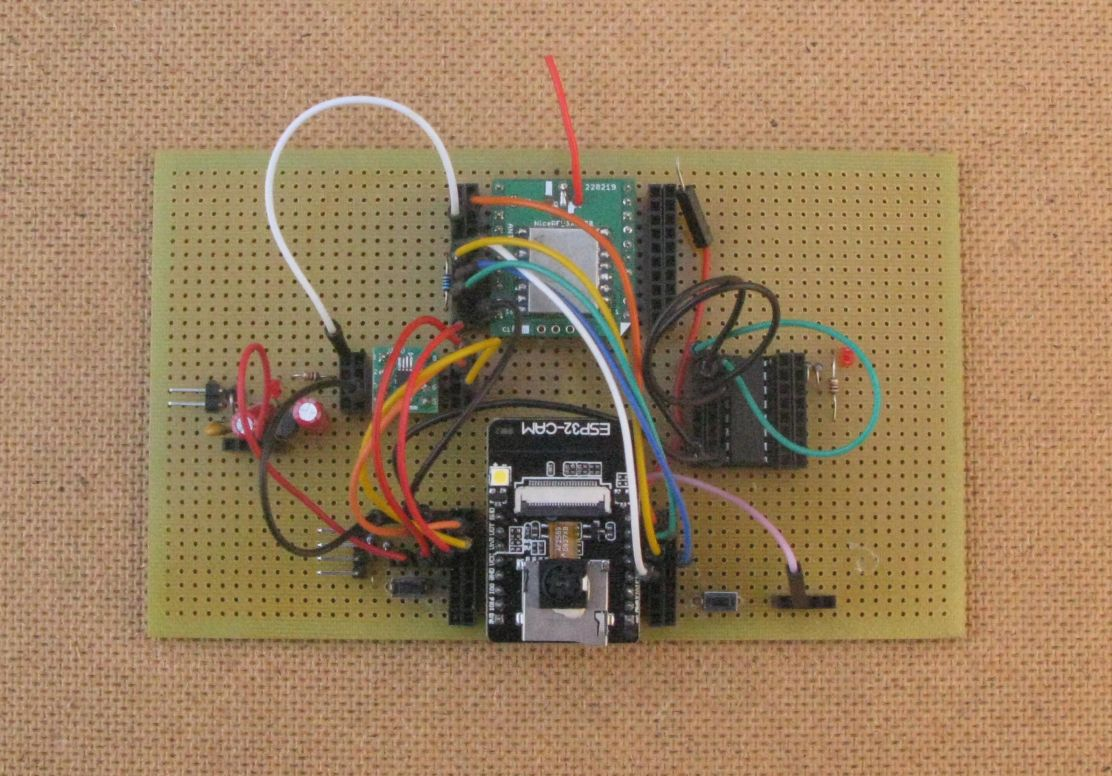
\includegraphics[width=0.85\textwidth]{sections/imagens/ESP32CAM_LoRa.jpg}
    \small
    \begin{quote}
        Fonte: \cite{robinson2021stuartcam}.
    \end{quote}
\end{figure}

\subsubsection{Getaways}

O gateway, como demonstrado na figura~\ref{fig:implementacao_tipica_lorawan}, é um elemento da rede LoRaWan que tem como responsabilidade agrupar dispositivos finais e viabilizar a comunicação entre o dispositivo final e o servidor de rede, \cite{Camargo2022}. 

A comunicação entre o dispositivo final e o gateway é realizada via protocolo LoRaWan, onde o gateway pode realizar a tarefa de registrar tráfego de mensagens. 
Como explicado por \citeonline{semtech2024an1200_86}, os dispositivos finais ao realizar o envio de uplink, distribuem as suas mensagens à todos os getaways alcançáveis dentro da mesma rede, tal função tem como objetivo garantir a que ao menos um dos gateways da rede receba e transmita a mensagem ao servidor de rede.

Os gateways operam em camada física, convencionalmente, assumem a responsabilidade apenas de viabilizar o tráfego de requisições uplink e downlink e realizar a verificação de integridade do pacote, não realizando processamento intermediário da mensagem para enviá-la ao servidor de rede, \cite{semtech2024an1200_86}.

A comunicação entre o gateway e o servidor de rede, corriqueiramente, é estabelecida utilizando protocolo TCP/IP. Toda comunicação dentro do protocolo LoRaWan é bidirecional, \cite{Camargo2022}.

É possível encontrar gateways prontos de multiplos canais sendo comercializados, mas é plenamente viável desenvolver getaways a partir de módulos e placas de prototipagem como a apresentada na figura~\ref{fig:esp32cam_lora}. 

\subsubsection{Servidores de Rede e Aplicação}

Como apresentado por \citeonline{Camargo2022}, servidores de rede e servidores de aplicação, dado a estrutura em que foram desenvolvidos, tanto podem ser implementados sob o mesmo hardware, como podem estar fisicamente distantes, realizando comunicação através de protocolo TCP/IP.

Servidores de rede são responsáveis por receber, descartar duplicatas e descriptografar mensagens enviadas por uplink. Outra responsabilidade do servidor de rede é realizar a configuração de dispositivos finais através de requisições downlink.

Servidores de Aplicação são responsáveis por receber pacotes enviados pelo servidor de rede, tratar e disponibilizar ao usuário as informações extraídas pelos dispositivos finais.

Ambos tipos de servidores possuem soluções prontas para implementação tanto em servidor local, como em nuvem. Entre eles destacam-se xxx que tem como característica xxxx e xxx que aplica-se sob o cenário xxxx.

